\documentclass[12pt]{article}
\usepackage{geometry}
\geometry{letterpaper, left=22.5mm, right=22.5mm, top=30mm, bottom=30mm}
\geometry{letterpaper}
\usepackage{amsmath}
\usepackage{amssymb}
\usepackage{enumitem}
\usepackage{fancyhdr}
\usepackage{framed}
\usepackage{tikz}
\usepackage{mathpazo}
%\usepackage{charter}
%\usepackage{newcent}
\usepackage{indentfirst}
\usepackage{booktabs}
\usepackage{graphicx}
\usepackage{float}
\usepackage{makecell}
\usepackage{xcolor}
\usepackage{mdframed}
\usetikzlibrary{trees}
\pagestyle{fancy}
\usepackage{amsthm}
\theoremstyle{definition}
\newtheorem{definition}{Definition}[section]
\theoremstyle{property}
\newtheorem{property}{Property}[section]
\theoremstyle{assumption}
\newtheorem{assumption}{Assumption}[section]
\theoremstyle{example}
\newtheorem{example}{Example}[section]
\theoremstyle{comment}
\newtheorem{comment}{Comment}[section]
\newtheorem{theorem}{Theorem}[section]
\newtheorem{corollary}{Corollary}[theorem]
\newtheorem{lemma}[theorem]{Lemma}
\usepackage{lastpage}
\usepackage{wrapfig}
\usepackage{hyperref}
\usepackage{subcaption}
\usepackage{setspace}
\hypersetup{
colorlinks=true,
linkcolor=black,
filecolor=green, 
urlcolor=blue,
}
\newcommand{\ROM}[1]
    {\MakeUppercase{\romannumeral #1}}
\fancyhead[L]{Econometrics \ROM{2}: Recitation 13 }%change each reci
\fancyhead[R]{Spring 2020}
\fancyfoot[C]{\thepage \hspace{1pt} / \pageref{LastPage}}

\fancypagestyle{firstpage}{%
\fancyhf{}%
\renewcommand{\headrulewidth}{0mm}%
  \fancyfoot[C]{\thepage \hspace{1pt} / \pageref{LastPage}}
}
%change title each rec
\title{Introduction to Econometrics \ROM{2}: Recitation 13\footnote{This is based on the lecture notes of Professors Jushan Bai and Bernard Salanie. I was also greatly helped by previous recitation notes from Paul Sungwook Koh and Dong Woo Hahm. The remaining errors are mine. }}

\begin{document}
\linespread{1.25}
\onehalfspacing

\author{Seung-hun Lee\footnote{Contact me at \href{mailto:sl4436@columbia.edu}{sl4436@columbia.edu} if you spot any errors or have suggestions on improving this note.}}
\date{May 9th, 2020}
\maketitle
\thispagestyle{firstpage}

%%%%%%%%%%%%%%%%%%
\section{Machine Learning}
\subsection{Random Forests}
Random forests use a series of decision trees - a stack of two-way splits with several number of depths - to solve a classification problem. The splits are based on covariate $k$ being above or below a certain threshold. The process stops at some depth and predict with the mean of $y$ at the terminal node $x$ belongs to. The covariate and the threshold combination that determine the split are selected so as to have the largest separation possible. This is commonly referred to as a `greedy' way of creating random forests.  \par
The detailed way of constructing random forests are as follows. Randomness is injected in several levels: one to select a random sample to train each tree on. Second level of randomness is involved in selecting variable candidates to determine splits for the trees. At the end, we get a prediction for any $x$, average of the predictors of the trees. We can also estimate the prediction error at any observation $x_i$ and gain expected prediction error overall. We can also identify which covariates contributed the most the the prediction using the variance-importance plots. This is where the random forests gain the advantage of interpretability - explaining as to why the results of the prediction came out to be as it is (not just spitting out the number). \par
There are some trade-offs. We want some level of depths in order to reduce the variance in the prediction and get a better fitting. However, too much depth will lead to overfitting. It is usually very difficult to find the happy medium. \par
Below is the example of the decision brought from Varian (2014). A random forests would be obtained by multiple trees, each with different sample (selected through bootstrap) and different variable and threshold combination. 
\begin{figure}[H]
\centering
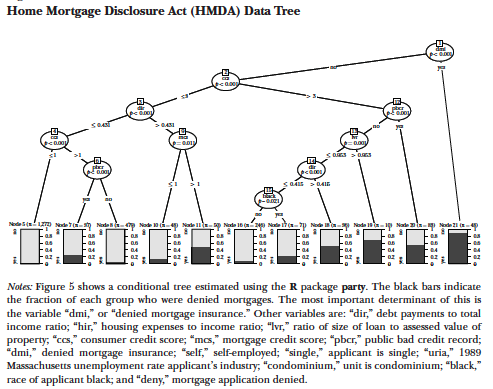
\includegraphics[width=0.7\textwidth, keepaspectratio]{randomforest.png}
\caption{From Varian (2014), Figure 5}
\end{figure}\par
\subsection{Double Machine Learning De-biasing Technics}
Often we are interested in testing for regarding the value of the parameter of interest. For instance, the average treatment effect under the conditional independence assumption. Specifically, we assume $(\epsilon_i(1),\epsilon_i(0))\perp\!\!\!\perp u_i|X_i$ where $X_i$ contains a large set of covariates. What we may do is to estimate the propensity score using machine learning techniques such as LASSO. Then, estimate the average treatment effect with the formula of our choice. Ideally, we want to conduct some standard tests. \par
Here is the problem - what we have for the propensity score is an estimate with some error. So depending on the size of this error, the estimate of the average treatment effect could be affected. Moreover, the propensity score is just a means towards our ultimate goal of obtaining the average treatment effect - it is merely a nuisance parameter. Since what we are doing involves errors at two different stages, we need a double machine learning de-biasing technics. Specifically, we decouple the propensity score and the treatment effect by applying Neyman Orthogonalization. In principle, what this method allows us to do is to do a two-step estimation by getting the estimate for the propensity score and then estimate the ATE without having to worry too much about the contaminated standard errors originating from the fact that we are not using the exact the propensity score. \par
In our case, what we can do is to
\begin{enumerate}
\item Split data into $K$ folds
\item Use LASSO to estimate $\hat{P}_k=\Pr(D_i=1|X_i)$ in all folds except the $k$th one. $k$ can be from 1 to $K$. 
\item If we are using inverse probability weighting method, for instance, we can get
\[
\widehat{ATE}=\sum_{k=1}^K\left[\frac{\sum_{i\in k}\frac{Y_iD_i}{\hat{P}_k(X_i)}}{\sum_{i\in k}\frac{D_i}{\hat{P}_k(X_i)}}-\frac{\sum_{i\in k}\frac{Y_i(1-D_i)}{1-\hat{P}_k(X_i)}}{\sum_{i\in k}\frac{(1-D_i)}{1-\hat{P}_k(X_i)}}\right]
\]
and use standard asymptotics to conduct tests. 
\end{enumerate}
\section{Finals Review: List of Important Topics}
\subsection{Bootstrap and Multiple Testing}
\begin{itemize}
\item \textbf{Better ways to do asymptotics:} There are cases when we are not certain about the characteristics of the distribution that generated the data. There are cases where we only know the asymptotic properties and not much about the finite sample properties. In this context, taking an asymptotic approach can lead to inaccurate estimations. \par
Therefore, we can look into conducting a bootstrap estimation, which is at least as better as classical asymptotics and sometimes better. Bootstrap estimation is also consistent and under some conditions, they have smaller approximation error. \par
We can conduct bootstraps by getting an IID sample $(X_1,...,X_n)$ from the data and treating this as a population sample. We obtain a $t$-statistics from this sample. We make $n$ draws with replacement and compute the new $t$-statistics. Re-draw the sample as many times as you like and keep track of each $t$-statistic. Then, generate an empirical distribution of these statistics and identify relevant cutoffs, $(2.5\%$ and $97.5\%)$ for instance, that can be used to create upper and lower bounds for the bootstrap confidence intervals. It can be shown, using Edgeworth expansion, that bootstrap approximation error and the classical approximation error have the same size of error, $O\left(1/\sqrt{n}\right)$. If the test statistic is (asymptotically) pivotal, then bootstrapped estimation can do better since they have smaller approximation error of $O\left(1/n\right)$.

\item \textbf{Proper ways to run multiple tests:} When we are conducting multiple hypothesis tests naively, we can run into a mistake of making a false discovery - rejecting a true null hypothesis. This can be dangerous even if we can assume that each hypotheses are independent of each other, as we might end up rejecting a null hypothesis ``just out of pure luck". \par
There are two approaches to multiple testing. One is to control for familywise error rate. Bonferroni and Holm method falls into this category. Bonferroni method uniformly applies a lower $p$-value cutoff below which the hypothesis is rejected. Holm method is a step-down method that considers from the hypothesis with the lowest $p$-value to the highest one. Generally, the cutoffs in Bonferroni method is lower than those of Holm method, making it a more conservative approach. However, in showing how these were, we were able to show that they did not depend on the (in)dependence structure of the hypotheses. \par
Another method controls for false discovery rate. We have learned the Benjamini - Hochberg method, which can be considered as a step-up method in the sense that we order hypotheses from the lowest $p$-value to the highest and start from the hypothesis with the highest $p$-value. Graphically, we plot the actual $p$-values of each hypotheses and the relevant cutoff $p$-values used to reject/not reject the null hypothesis. We check whether the actual $p$-value lies above the cutoff, accept that $H_0$ as true and move on to the next highest hypothesis. The process is stopped when the actual $p$-value starts to lie below the cutoff $p$-value. The remaining hypotheses are all considered to have a false $H_0$. 
\end{itemize}

\subsection{Quantile Regression}
\begin{itemize}
\item \textbf{Not everything is about conditional means:} Up until this point, we were obtaining conditional expectation $E[Y_i|X_i]$ from the regressions. However, we may be interested in not just the conditional expectation, but some other distributional properties. For instance, what is the effect of a job training program to those whose baseline income was at around the median of the income distribution? To answer this, we run a quantile regression that is meant to capture different values of the parameter of interest depending on the location of the conditional distribution. 
\par
In running quantile regression, check function is very useful. The check function $\rho_\tau(u)$ is defined as
\[
\rho_\tau(u)=u(\tau-1(u\leq0))
\]
$\tau\in[0,1]$ is the point in the distribution we are interested in. In estimation, $u$ can be replaced by $Y_i-X_i\beta$. For any value of $\tau$, there is going to be a kink for the check function at $u=0$. We make use of this property and obtain the quantile estimator by minimizing 
\[
E[\rho_\tau(Y_i-X_i\beta)|X_i] \text{ or }E[\rho_\tau(Y_i-X_i\beta)X_i]
\]
\end{itemize}
\subsection{Nonparametric Regression}
\begin{itemize}
\item \textbf{Why do we even do this?} We rarely have the exact knowledge about the characteristics of the distribution $P(y|x)$ that the observations are drawn from. When we carry out nonparametric estimation, we are not required to make any modeling assumptions related to the data. This helps address one of the key internal validity threats - using the wrong functional forms in the specification. We can also use nonparametric regression in tandem with parametric estimation. Run the model parametrically and run the same model in nonparametrics to confirm whether our parametric form is correct
\item \textbf{Bandwidth is essential!} In theory, there are two things to consider when setting up nonparametrics - form of the kernel density estimation and the bandwith. The former does not impact the result as much (so I will discuss using uniform kernel). The density estimation for function $f$ can be written as
\[
\hat{f}(x)=\frac{1}{nh}\sum_{i=1}^n K\left(\frac{x-X_i}{h}\right)
\]
where $K(\cdot)$ is the kernel density estimator of our choice. 
\par 
Bandwidth, on the other hand, is essential. There are different consequences for undersmoothing and oversmoothing. When we undersmooth, we are including more variation than necessary and computation becomes difficult. When we oversmooth, we risk dropping even the essential traits about the distribution and mis-estimate the true density. The key to finding the optimal bandwidth is to balance between the bias and the variance. Wider bandwidth increases bias but decreases variance. Narrower bandwidth does the opposite. The answer can be found by minimizing the asymptotic mean integrated square error (AMISE)
\[
\int E(\hat{f}(x)-f(x))^2dx
\]
where $E(\hat{f}(x)-f(x))^2$ can be written as the sum of variance and bias$^2$. In practice, we can choose the bandwidth based on Silverman's rule of thumb or from cross-validation. 
\item \textbf{So what are the gains?} One of the nonparametric methods we can use is local constant (Nadaraya and Watson Estimator), local linear, or local polynomial estimation. Key gains from nonparametrics compared to parametric estimation is the flexibility in the sense that the type of association between the covariates and the dependent variable is not bound by the functional form selected in parametric approach. We can model flexible relationship with just nonparametric estimation (albeit with some errors, which is why having a confidence interval is necessary).
\item \textbf{The cost?} The cost of nonparametric estimation could be big if you are using a large dataset with many covariates. This is known as curse of dimensionality. This refers to the fact that as the dimension of covariates become larger, larger sample size is required to do any sort of asymptotic inference. Put it differently, the estimators converge to its asymptotic values in a much slower pace than in parametric setup. Curse of dimensionality can kick in even if we have just a slightly more than a handful of covariates to regress. \par
One of the middle grounds that is used in an attempt to have both traits of nonparametric and parametric regression is the semiparametric regression. In class, we learned partially linear models where we run
\[
Y_i = X_i\beta + g(W_i)+\epsilon_i
\]
$X_i$ covariates inherit the characteristics from the parametric regression while $W_i$ covariates are similar to nonparametric regression. 
\end{itemize}
\subsection{Treatment Effects}
\begin{itemize}
\item \textbf{Fundamental Problem in Treatment Effects:} What we are interested in how a treatment changes the outcome of interest $Y$ for individual $i$, that is
\[
Y_i(1)-Y_i(0)
\]
Unfortunately, there are always a problem of a missing data - you cannot be treated and untreated at the same time. Specifically, if we are to identify what an average treatment effect is,
\begin{align*}
E[Y_i(1)-Y_i(0)]&=\Pr(D_i=1)E[Y_i(1)|D_i=1]+\Pr(D_i=0)\textcolor{red}{E[Y_i(1)|D_i=0]}\\
&-\Pr(D_i=0)E[Y_i(0)|D_i=0]-\Pr(D_i=1)\textcolor{red}{E[Y_i(0)|D_i=1]}
\end{align*}
We can get all the other conditional expectations from the data except the ones in red. Without making any assumptions, we cannot even calculate what the average treatment is. The type of assumptions we set determine what the conditional expectation in red can be expressed as. We may be luck to have a random assignment, where treatment is assigned in a purely random fashion. If not, we may be able to condition the treatment status on some covariates, and the potential outcomes would be random conditional on treatment conditioned by some covariates. This type of situation is called selection on observable.\par
There might also be some other problems beyond the missing data problem. Specifically, the treated population and the untreated population may be different in some unobservable dimensions. In such case, conditioning the outcome on the treatment status alone would not give us an accurate assessment of the treatment effect. In such case, we are left to rely on instrumental variables to back out the treatment effect. Marginal treatment effects and local average treatment effect falls into this category.\par
Depending on the assignment mechanism used, we may be able to use this to our advantage. If the assignment was based on some sort of a cutoff, then there is bound to be a jump in probability of being treated. This discontinuity allows us to utilize regression discontinuity, one of the front-runner methods in applied economics. 
\item \textbf{Assumptions} 
\begin{itemize}
\item Random assignment: This is a very ideal case. In this situation, all we need to assume is that the potential outcome is independent of treatment assignment status. Specifically, 
\[
(Y_i(1), Y_i(0)) \perp\!\!\!\perp D_i
\]
What this implies is that
\[
E[Y_i(d)|D_i=d]=E[Y_i(d)|D_i=d']=E[Y_i|D_i=d]
\]
where $d=0,1$ and $d'=\begin{cases} 1&(d=0)\\ 0 & (d=1)\end{cases}$ and the last equation is from the potential outcome framework $Y_i=Y_i(1)D_i+Y_i(0)(1-D_i)$.
\item Conditional independence assumption: Here, we assume that the potential outcomes are independent of $D_i$ but conditional on the additional covariates $X_i$. In math, we write, 
\[
(Y_i(1), Y_i(0)) \perp\!\!\!\perp D_i|X_i
\]
where $D_i=1(u_i<p(X_i))$. Loosely speaking, $p(X_i)$ is the propensity score and the $u_i$ indicates to resistance to entering treatment, distributed $U[0,1]$. Or
\[
E[Y_i(d)|D_i=d, X_i=x]=E[Y_i(d)|D_i=d', X_i=x]=E[Y_i|D_i=d, X_i=x]
\]
\item Selection on unobservables: Here, the potential outcome is no longer independent of $D_i$, even if conditioned on $X_i$. Instead, we need to find an instrument $Z_i$ that satisfies two conditions. The $Z_i$ should be relevant to the treatment status $D_i$  (or the propensity score) and the monotonicity condition. $Z_i$ should satisfy the validity condition s.t.
\[
(Y_i(1), Y_i(0), u_i) \perp\!\!\! \perp Z_i|X_i
\]
where $u_i$ is the resistance to being treated parameter. \par
To run marginal treatment effect, the instrumental variable $Z_i$ should have a continuous support. In addition, it would also be ideal to have the propensity score take the value from $[0,1]$. For local average treatment effect,  we would not necessarily require $Z_i$ to be continuous. A binary variable for a $Z_i$ would be sufficient. \par
Due to the monotonicity condition for both cases, the defiers are not included. As such, we begin to lose some number of samples as we use instruments. This could potentially hurt the external validity of the treatment estimates. 
\item Regression discontinuity: Unlike previous cases, overlap of the covariates to treatment status is not too essential, as sharp RD does not involve any overlap. However, there are some conditions that should be met. One is that propensity score should jump around the cutoff of the forcing variable. Second is that all the covariates should remain continuous around the cutoff. Third is that there should be no bunching of the forcing variable at the cutoff. Lastly, the continuity of the potential outcome in the sense that 
\[
E[Y_i(d)|X_i, W_i=c^+]=E[Y_i(d)|X_i, W_i=c^-]=E[Y_i(d)|X_i, W_i=c]
\]
\end{itemize}
\item \textbf{Identification Tactics}
\begin{itemize}
\item Random assignment: In this case, we have $E[Y_i(d)|D_i=d]=E[Y_i(d)|D_i=d']$. So we can back out the average treatment effect on all population. Specifically, 
\begin{align*}
E[Y_i(1)-Y_i(0)]&=\Pr(D_i=1)E[Y_i(1)|D_i=1]+\Pr(D_i=0)E[Y_i(1)|D_i=0]\\
&-\Pr(D_i=0)E[Y_i(0)|D_i=0]-\Pr(D_i=1)E[Y_i(0)|D_i=1]\\
&=E[Y_i|D_i=1]-E[Y_i|D_i=0]
\end{align*}
\item Conditional independence assumption: In assuming conditional independence, what we can back out is the average treatment effect for those whose $X_i=x$. Specifically
\begin{align*}
E[Y_i(1)-Y_i(0)|X_i=x]&=E[Y_i(1)|D_i=1, X_i=x]-E[Y_i(0)|D_i=0, X_i=x]\\
&=E[Y_i|D_i=1, X_i=x]-E[Y_i|D_i=0, X_i=x]\\
\end{align*}
\item Selection on unobservables: For marginal treatment effect, its theoretical definition and the equivalent expression obtainable from the data is
\[
MTE(p)=E[Y_i(1)-Y_i(0)|u_i=p, X_i]=\frac{\partial E[Y_i|p(x,z)=p, X_i]}{\partial p}
\]
The equivalence between the two expression is stated in both the lecture notes and the recitation notes. \par
For the local average treatment effect, the definition and the equivalent expressions are
\small{\[
LATE(x)=E[Y_i(1)-Y_i(0)|p(x,z)<u_i<p(x,z'),X_i]=\frac{E[Y_i|Z_i=z',X_i]-E[Y_i|Z_i=z,X_i]}{E[D_i|Z_i=z',X_i]-E[D_i|Z_i=z,X_i]}
\]}\normalsize
You can refer to the recitation notes to see why they are equivalent. \par
In both cases, we are only observing the treatment effect on the compliers. What is being observed is those who change their treatment status from 0 to 1 as we move the propensity scores. So always takers and never takers are not considered. Monotonicity rules out defiers. 
\item Regression discontinuity: What we are identifying with the RD framework is the average treatment effect for the observations within the bandwidth around the cutoff of the forcing variables. Generally speaking, we use the fact that
\footnotesize{\begin{gather*}
E[Y_i|X_i, W_i=c^+]=E[Y_i(0)|X_i, W_i=c^+]+\Pr(D_i=1|X_i, W_i=c^+)E[Y_i(1)-Y_i(0)|X_i, W_i=c^+]\\
E[Y_i|X_i, W_i=c^-]=E[Y_i(0)|X_i, W_i=c^+]+\Pr(D_i=1|X_i, W_i=c^-)E[Y_i(1)-Y_i(0)|X_i, W_i=c^-]
\end{gather*}}\normalsize
after some algebra (included in the recitation note), we can back out
\footnotesize{\[
E[Y_i|X_i, c^+]-E[Y_i|X_i, c^-]=[\Pr(D_i=1|X_i, c^+)-\Pr(D_i=1|X_i, c^-)]E[Y_i(1)-Y_i(0)|X_i,c]
\]}\normalsize
So we do identify
\[
E[Y_i(1)-Y_i(0)|X_i,c]=\frac{E[Y_i|X_i, c^+]-E[Y_i|X_i, c^-]}{\Pr(D_i=1|X_i, c^+)-\Pr(D_i=1|X_i, c^-)}
\]
which is an average treatment effect for a very small group of observations-those within the bandwidth around $W_i=c$. If we are in a sharp RDD framework, the denominator is just 1. This is also similar to LATE in intuition and math if we let $Z_i=1(W_i\geq c)$ and in that they identify treatment effect for compliers only.
\end{itemize}
\item \textbf{Implementation}
\begin{itemize}
\item Random assignment: Conducting an OLS regression in the model
\[
Y_i = \beta_0+\beta_1D_i+u_i
\]
would get us an unbiased estimate of $\beta_1$,  which is the treatment effect. Note that
\[
E[Y_i|D_i=0]=\beta_0,\ \ \ E[Y_i|D_i=1]=\beta_0+\beta_1
\]
\item Conditional independence assumption: There are many approaches here. One of them is a matching estimation where we match between observations in different treatment arms that share a similar $X_i$ values. However, this method is sensitive to the choice of the number of neighbors we allow and in some cases, distance measure. \par
Another method is to use inverse probability weighting method, where those who are treated are weighted by $\frac{1}{p(x)}$ and those in the control are weighted $\frac{1}{1-p(x)}$. The magic formula mentioned in the lecture falls into this category\par
Difference in differences also belong to this case. The idea is that the treatment and controlled are equally untreated before a certain period but the former group is treated after a certain period (denoted as $T$). Using this assignment mechanism, we can regress
\[
Y_{it}=\beta_0(X_i)+\beta_1(X_i)\cdot1(t\geq T)+\beta_2(X_i)\cdot1(i\in D_i)+\beta_3\cdot1(t\geq T)\cdot1(i\in D_i)+\epsilon_{it}
\]
\item Selection on unobservables: For marginal treatment effects, we can do it parametrically in the following way. Estimate the propensity score by regressing $D$ on $X$ and $Z$. Then, using the propensity obtained, regress $Y$ on $X$ and the propensity score flexibly. For instance, include a term that interacts propensity and $X$ and higher powered terms of the propensity score. This allows us to check whether the CIA is satisfied by looking at the coefficient and $p$-values of the $p^2$ and above terms. For a nonparametric approach, use a local linear estimation and in particular, look at the coefficient in front of the linear term. \par
For local average treatment effect, regress $D$ on $Z$ and other covariates. Then regress $Y$ on $X$ and the predicted $D$. This two-stage-least-squares approach yields local average treatment effect from the Wald estimator. 
\item Regression discontinuity: Nonparametrically, we can fally Calonico et al. (2014) by running a local polynomial on $[c-\epsilon,c
)$ and $[c,c+\epsilon]$ and select the bandwidth in the manner of Imbens and Kalyanaraman. The key is that the domain of regression should not overlap between the area below $c$ and above $c$ or we risk misfitting. \par
Parametrically, we can run regressions separately above and below the cutoff to capture different trends. Or run the following equation at the whole sample
\small{\[
Y_i=X_i\beta + X_i\cdot 1(W_i\geq c)\gamma+X_i\cdot (c-W_i)\delta+ X_i\cdot (c-W_i)\cdot 1(W_i\geq c)\mu+\epsilon_i
\]}\normalsize
\end{itemize}
\end{itemize}
%%%%%%%%%%%%%%%
\end{document}

